\documentclass[a4paper,12pt]{article}
\usepackage{graphicx}
\begin{document}

\centerline{\huge \textbf{Requirements documentation}} \hspace*{\fill}
\\
The goal is to make an optimized solution for finding the shortest path in a vector-based geometry. The program will assume that geometry is Euclidean, that way the shortest possible path between two points is assumed to be a straight line.
\paragraph{Required algorithms} \hspace{0pt} \\
Instead of dividing the geometry into pixels, here points will be placed in a two-dimensional
coordinate, that will then be joined to form a chain of edges. Edges are then required to form
a loop - in other words - a shape. This shape can then be interpreted as a wall or a non-wall.
\\
\centerline{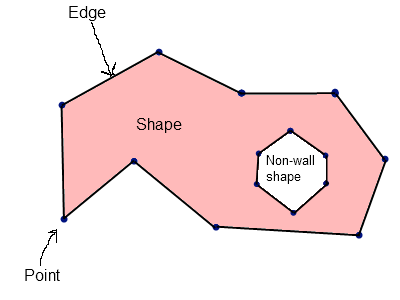
\includegraphics[scale=0.5]{pointedgeshape.png}} \hspace*{\fill}
\\
Each point in the vector field is connected to two other points. That way each point can be considered as an angle between the non-wall part.
\\
\centerline{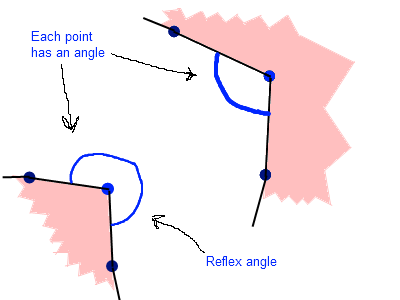
\includegraphics[scale=0.5]{pointsandangles.png}} \hspace*{\fill}
\\
\\
Pathfinding algorithm generates the shortest available path from point A to point B,
avoiding possible walls along the way. Algorithm will construct a graph from the vector field.
All points whose angles are reflex (between 180$^\circ$ and 360$^\circ$) are vertices in the graph. Points A and B are vertices as well. Edges in the graph have a value, which is a distance between two vertices calculated by Pythagerous' theorum. That way an edge value can't be less than zero. With this graph the shortest path between points A and B can be found using the Dijkstra's algorithm.
\\
\\
\centerline{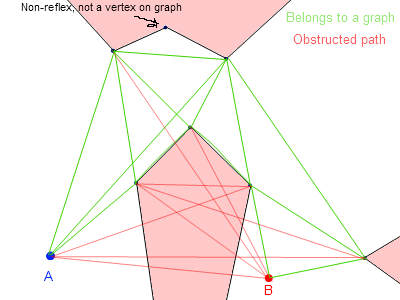
\includegraphics[scale=0.65]{graph.png}} \hspace*{\fill}
\\
\\
Two points are connected in the graph if the path between these points is unobstructed.
Because of this, the project will require a tracing algorithm. Current idea of the algorithm is taking each point and mapping a maximum distance for all of its directions.
\\
\\
\centerline{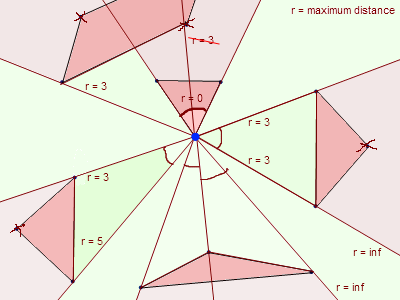
\includegraphics[scale=0.6]{trace.png}} \hspace*{\fill}
\\
\\
The project will provide a relatively user-friendly tool for geometry manipulation. This tool will imitate a brush of a certain width, leaving a track with each stroke of a computer mouse. The stroke either creates a wall shape, or erases a piece of wall from the field. Straight-forward point manipulation via point dragging will be provided as well.
\paragraph{Resource requirement} \hspace{0pt} \\
Main focus in the project is on optimization. Pathfinding algorithm should work on run-time in
modern middle-end computers. Editing the vector field and repositioning the destination point
should work on run-time as well. These requirements should apply with relatively complex geometry.
\\
\\
Graph generation will require a time resource of $O(n^2)$, where n is amount of points with reflex angles. That's because each point should check whether they can be connected with all of the other points. Graph generation will be called every time the vector field is modified. This can be optimized by making the algorithm reconstruct the graph at regions where vector field was modified, instead of rebuilding the whole graph.
\\
\\
If source and destination points are changed, graph shouldn't be reconstructed completely. In that case algorithm should check which points are reached from points A and B, which makes the algorithm's time resource $O(n)$.
\\
\\
Path finding on the generated graph will requires the same time resource as in Dijkstra's algorithm: $O((v+e)*log(v))$, where v is amount of vertices in the graph and e is amount of edges in the graph. The graph's density will vary, which is why the value of e can't be assumed to be close to either n or $n^2$.
\\
\\
Field manipulation tool's time resource is hard to estimate. Most likely it's $O(n^2)$, because stroke overlapping has to be checked.
\\
\\
All of the points in the field have to be stored in the memory. Each point stores two other points with which it forms an edge for the shape, requiring a linear memory resource. Each shape may have to be stored as well, however amount of shapes can't be more than amount of points. Graph will require its edges to be stored, making the memory involvement $O(v+e)$, where v is amount of vertices in the graph and e is amount of edges in the graph.
\\
\\
Overall performance can be optimized by dividing the field into several rectangular zones. Each zone stores edges that are located there. Because an edge can cross several zones, an edge may be stored redundantly, increasing memory resource. However this trick may speed up vector field modification and tracing.

\paragraph{Reference} \hspace{0pt} \\

Lecture notes of Tietorakenteet ja algoritmit course will be used as a reference for implementing the most commonly used datastructures and algorithms like heap and Dijkstra's algorithm. Some algorithms will be partially improvised without a specific reference. There may be some 'googling around' involved, which leads to blogs or forum posts on overflowstackexchange for example.

\end{document}